\section{Auswertung}
\subsection{Vorbereitende Experimente}
In einem ersten Schritt werden die Freqzuenzspektren von verschiedenen Anzahlen $50 \,\symup{mm}$ Zylindern im Bereich 
von $0,1 \, \symup{kHz}$ bis $12 \, \symup{kHz}$ mit dem Oszilloskop aufgenommen. Zusätzlich wird die selbe
Messung mit dem PC aufgenommen; dies ist in \autoref{fig:blub1} dargestellt. Alle anderen Darstellungen sind
\autoref{fig:anhang1} bis \autoref{fig:anhang3} zu entnehmen.

\begin{figure}
    \centering
    \begin{subfigure}[b]{0.3\textwidth}
        \centering
        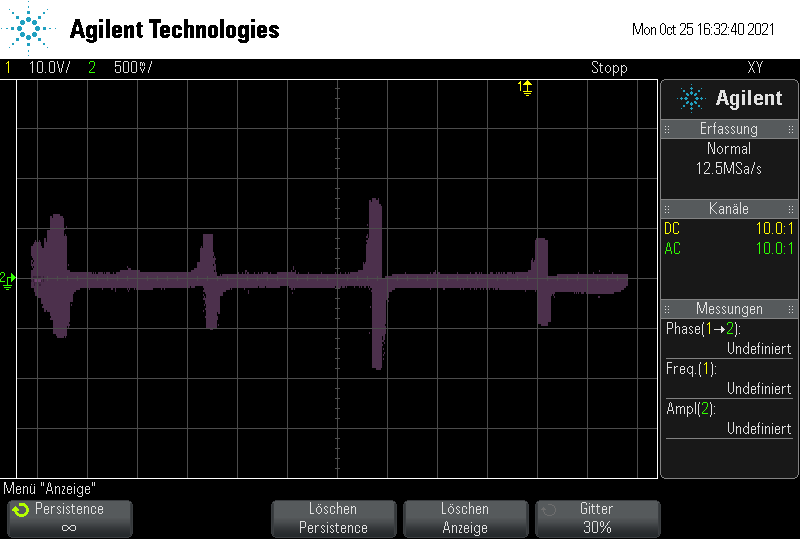
\includegraphics[width=\textwidth]{data/1_1zylinder50mm/scope_1.png}
        \caption{Oszilloskop, 1 Zylinder ($50 \, \symup{mm}$).}
    \end{subfigure}
    \hfill
    \begin{subfigure}[b]{0.3\textwidth}
        \centering
        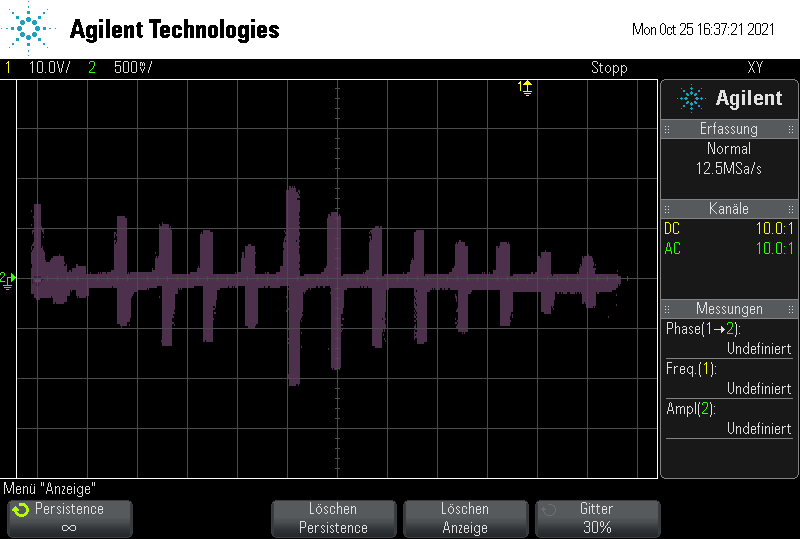
\includegraphics[width=\textwidth]{data/1_1zylinder50mm/scope_4.png}
        \caption{Oszilloskop, 4 Zylinder ($50 \, \symup{mm}$).}
    \end{subfigure}
    \hfill
    \begin{subfigure}[b]{0.3\textwidth}
        \centering
        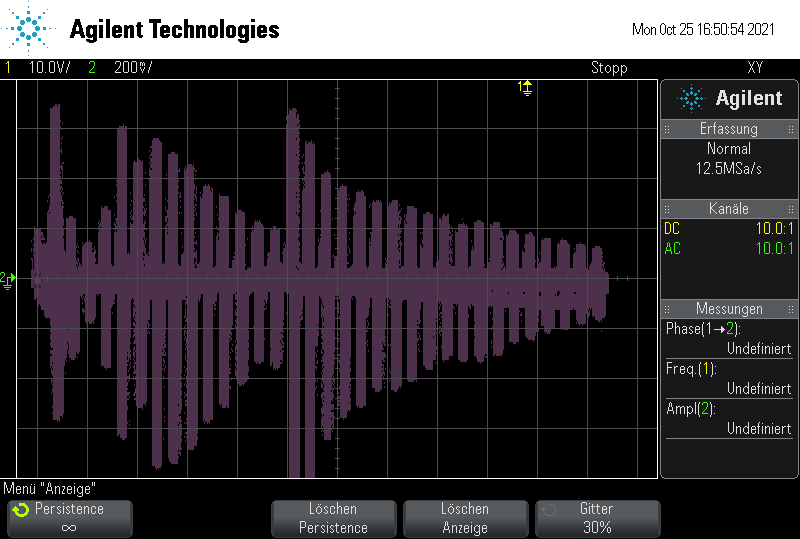
\includegraphics[width=\textwidth]{data/1_1zylinder50mm/scope_10.png}
        \caption{Oszilloskop, 10 Zylinder ($50 \, \symup{mm}$).}
    \end{subfigure}
    \hfill
    \begin{subfigure}[b]{0.3\textwidth}
        \centering
        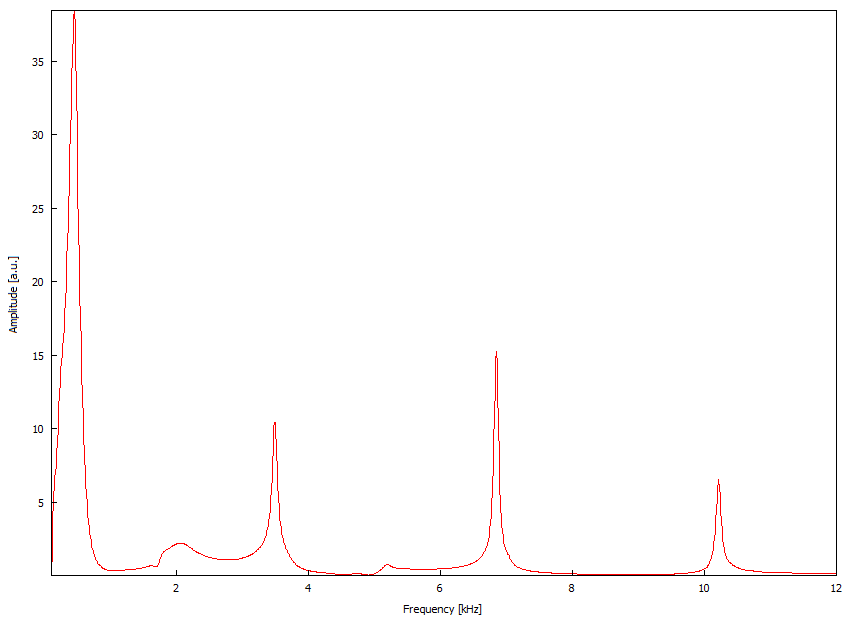
\includegraphics[width=\textwidth]{data/1_2zylinder50mmPC/1.png}
        \caption{PC, 1 Zylinder ($50 \, \symup{mm}$).}
    \end{subfigure}
    \hfill
    \begin{subfigure}[b]{0.3\textwidth}
        \centering
        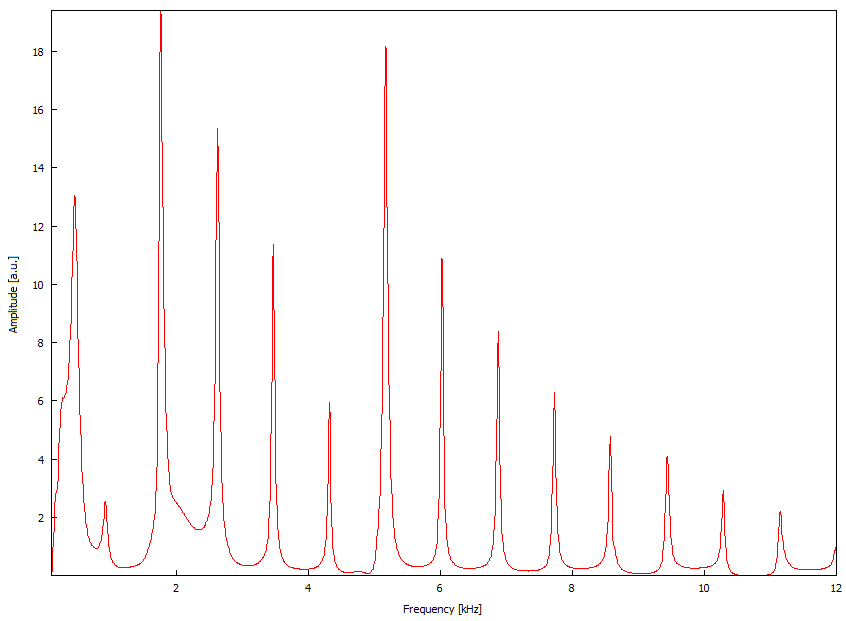
\includegraphics[width=\textwidth]{data/1_2zylinder50mmPC/4.png}
        \caption{PC, 4 Zylinder ($50 \, \symup{mm}$)}
    \end{subfigure}
    \hfill
    \begin{subfigure}[b]{0.3\textwidth}
        \centering
        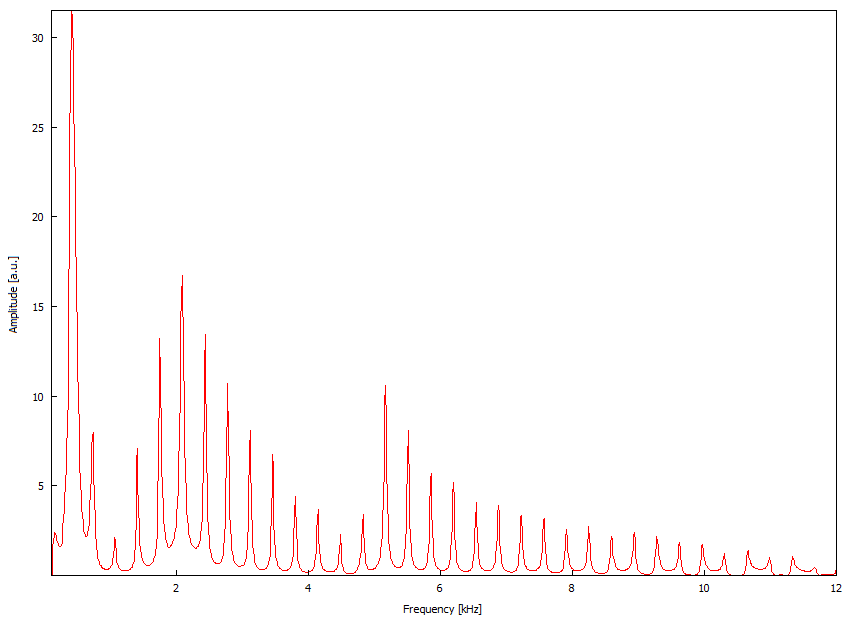
\includegraphics[width=\textwidth]{data/1_2zylinder50mmPC/10.png}
        \caption{PC, 10 Zylinder ($50 \, \symup{mm}$)}
    \end{subfigure}
       \caption{Das Frequenzspektrum von $0,1 \, \symup{kHz}$ bis $12 \, \symup{kHz}$ bei verschiedener Anzahl von Zylinder (Länge $50 \, \symup{mm}$) aufgenommen einmal mit einem Oszilloskop und einmal mit dem PC.}
       \label{fig:blub1}
\end{figure}

Es fällt auf, dass die Resonanzfrequenzen mit mehr Zylindern ebenfalls zunehmen. Des Weiteren stimmen die 
Darstellungen von Oszilloskop und PC überein. Die Artefakte im niedrigen Frequenzbereich treten bei beiden
Messreihen auf. Auch die Proportionalität der verschiedenen Resonanzfrequenzen ist bei den gemessenen
Spektren vergleichbar. Des Weiteren ist die Auflösung des PCs erwartungsgemäß höher als die des Oszilloskopes.\\
Abschließend wird noch ein weiteres Frequenzspektrum eines einzelnen $75 \, \symup{mm}$ Zylinders am PC aufgenommen.
Dieses ist in \autoref{fig:75mm1} dargestellt.
\begin{figure}[h]
    \centering
    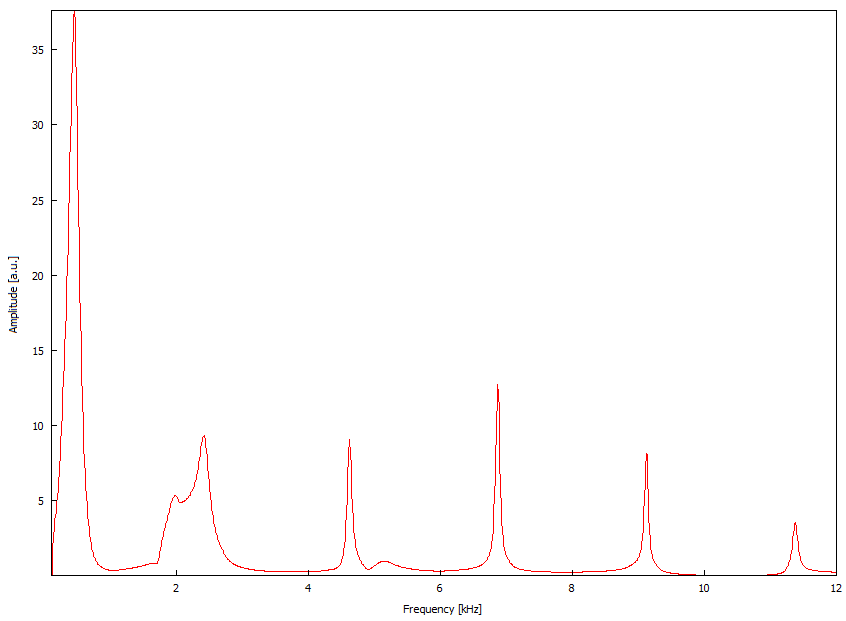
\includegraphics[width=0.6\textwidth]{data/1_3_zylinder75mm/1.png}
    \caption{Frequenzspektrum eines einzelnen $75 \, \symup{mm}$ Zylinders im Bereich $0,1 \, \symup{kHz}$ bis $12 \, \symup{kHz}$.}
    \label{fig:75mm1}
\end{figure}
Es wird deutlich, dass die Anzahl der Resonanzfrequenzen nicht von der Anzahl der Zylinder, sondern 
von der Länge des Gesamtzylinders abhängt. Die Anzahl der Peaks ist höher als bei einem $50 \; \symup{mm}$ Zylinder,
aber geringer als bei zwei $50 \, \symup{mm}$ Zylindern.

\subsection{Das Wasserstoffatom}
Das Frequenzspektrum des Wasserstoffmodells bei einem Winkel von $\alpha = 180°$ ist in \autoref{fig:hatom180}
dargestellt.
\begin{figure}[h]
    \centering
    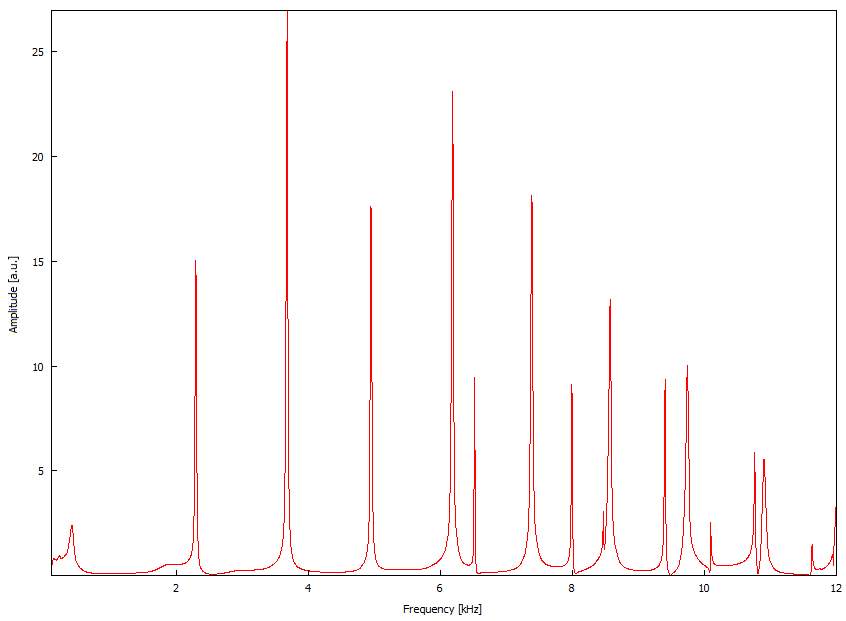
\includegraphics[width=0.6\textwidth]{data/2_1/180.png}
    \caption{Frequenzspektrum eines Kugelresonators bei einem Winkel von $\alpha = 180°$ im Bereich $0,1 \, \symup{kHz}$ bis $12 \, \symup{kHz}$.}
    \label{fig:hatom180}
\end{figure}

Vier der Resonanzfrequenzen wurden weiter nach Phasenverschiebung, Frequenz und Amplitude untersucht.
Die Daten sind in \autoref{tab:2_2} dargestellt. Auffällig ist, dass sich die Phasenverschiebung um die Resonzfrequenzen herum jeweils
sehr stark verändert und beim Durchlaufen des Frequenzspektrums mehrfach einen kompletten Kreis beschreibt.
Die Amplituden sind unterschiedlich hoch und nicht Deckungsgleich mit dem Spektrum in \autoref{fig:hatom180}.\\
\begin{table}[!htp]
    \centering
    \caption{Frequenzen, Amplituden, Phasenverschiebung und Ordnung einiger Resonanzfrequenzen.}
    \label{tab:2_2}
    \begin{tabular}{c c c c}
    \toprule
    {Ordnung} & {Resonanzfrequenz / kHz} & {Phasenverschiebung / °} & Amplitude \\
    \midrule 
    1  & 0,406 & -100 & 3,1\\ 
    2  & 2,279 &40 & 13,8 \\
    3  & 3,665 &-90 & 39,0 \\
    7  & 7,379 &165 & 42,6 \\
    \bottomrule
    \end{tabular}
    \end{table}

Für vier der Resonanzen wird nun die Druckamplitude als Funktion des Drehwinkels $\theta$ aufgestellt. Die hier 
verwendeten Resonanzfrequenzen sind die selben wie in \autoref{tab:2_2} beschrieben.
Der Drehwinkel $\theta$ ergibt sich dabei durch 
\begin{equation*}
    \theta = \text{arccos}\left(\frac{1}{2} \cos(\alpha) - \frac{1}{2}\right),
\end{equation*}
wobei $\alpha$ der Einstellwinkel des Kugelresonators ist.
Zudem werden die entsprechenden Kugelflächenfunktionen (\autoref{eq:kugelflaechen}) dargestellt
und Werte der Druckamplitude entsprechend der Kugelflächenfunktionen normiert.
Die Darstellungen der Winkelverteilungen der Amplituden und deren zugehörigen Kugelflächenfunktionen
sind in \autoref{fig:polar} dargestellt.
\begin{figure}
    \centering
    \begin{subfigure}[b]{0.45\textwidth}
        \centering
        \includegraphics[width=\textwidth]{build/Polar_04.pdf}
        \caption{1. Ordnung, $f = 0,406 \, \text{kHz}$.}
    \end{subfigure}
    \hfill
    \begin{subfigure}[b]{0.45\textwidth}
        \centering
        \includegraphics[width=\textwidth]{build/Polar_23.pdf}
        \caption{2. Ordnung, $f = 2,279 \, \text{kHz}$.}
    \end{subfigure}
    \hfill
    \begin{subfigure}[b]{0.45\textwidth}
        \centering
        \includegraphics[width=\textwidth]{build/Polar_37.pdf}
        \caption{3. Ordnung, $f = 3,665 \, \text{kHz}$.}
    \end{subfigure}
    \hfill
    \begin{subfigure}[b]{0.45\textwidth}
        \centering
        \includegraphics[width=\textwidth]{build/Polar_74.pdf}
        \caption{4. Ordnung, $f = 7,379 \, \text{kHz}$.}
    \end{subfigure}
    \hfill
    \caption{Die Amplitude des Drucks bei verschiedenen Resonanzfrequenzen $f$ in Abhängigkeit des Winkels $\theta$ mit den zugehörigen Kugelflächenfunktionen.}
    \label{fig:polar}
\end{figure}

Allgemein folgen die Amplituden des Drucks dem Verlauf der Kugelflächenfunktionen zumindest ungefähr.
Die größte Abweichung kann in der Resonanz 2. Ordnung beobachtet werden, in welcher die Amplituden
des Drucks dem Verlauf der Kugelflächenfunktion nicht mehr komplett folgen. Abweichungen gibt es
allerdings bei allen Resonanzfrequenzen, wobei erkennbar ist, dass dem Verlauf ungefähr gefolgt wird.\\
Mit dem eingesetzten Ringe von $3\, \symup{mm}$, $6\, \symup{mm}$ und $9\, \symup{mm}$ Größe ergibt sich ein Frequenzspektrum zwischen
$1,8 \, \symup{kHz}$ bis $2,3 \, \symup{kHz}$ bei einem Winkel von $\alpha = 180°$ wie in 
\autoref{fig:ringe} dargestellt.
\begin{figure}
    \centering
    \begin{subfigure}[b]{0.33\textwidth}
        \centering
        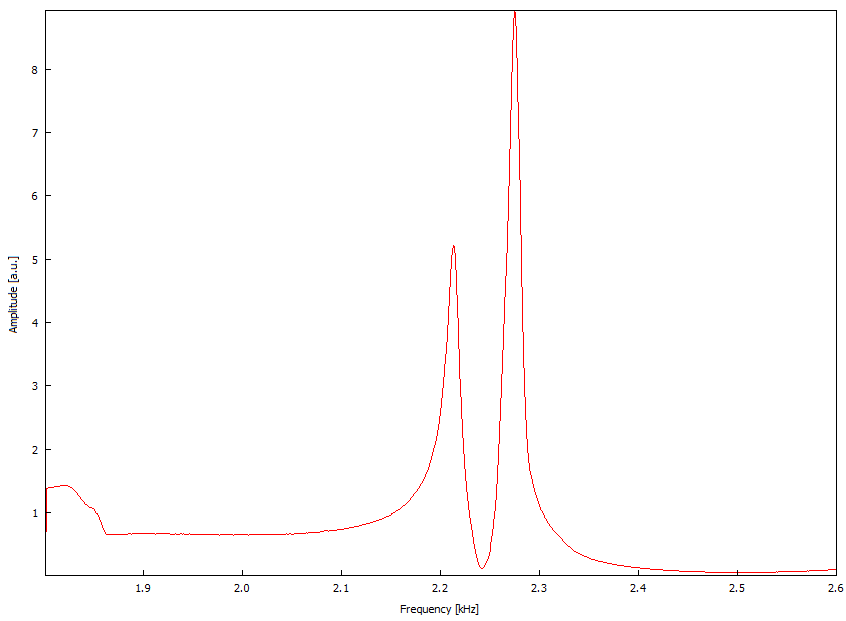
\includegraphics[width=\textwidth]{data/2_4/3mm.png}
        \caption{3\,mm Ring.}
    \end{subfigure}
    \hfill
    \begin{subfigure}[b]{0.33\textwidth}
        \centering
        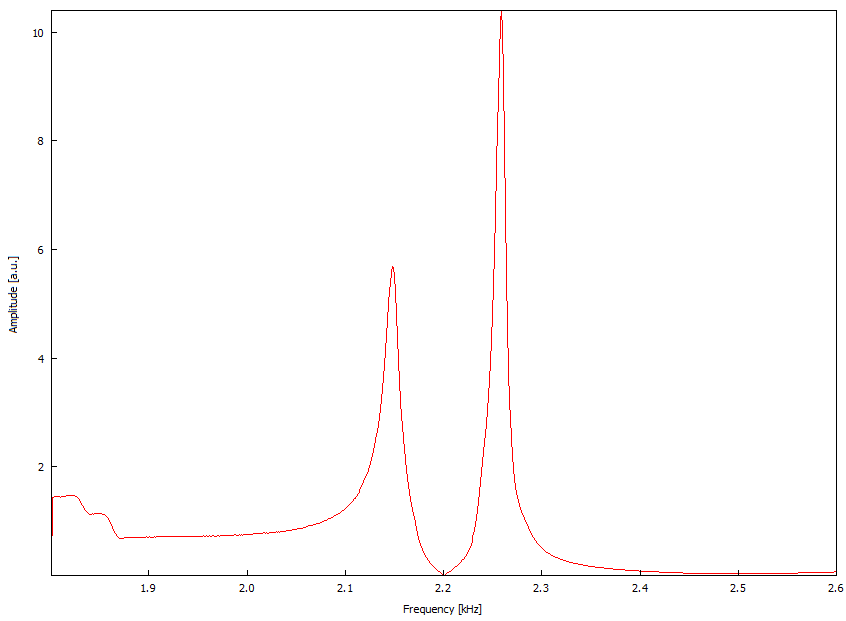
\includegraphics[width=\textwidth]{data/2_4/6mm.png}
        \caption{6\,mm Ring.}
    \end{subfigure}
    \hfill
    \begin{subfigure}[b]{0.33\textwidth}
        \centering
        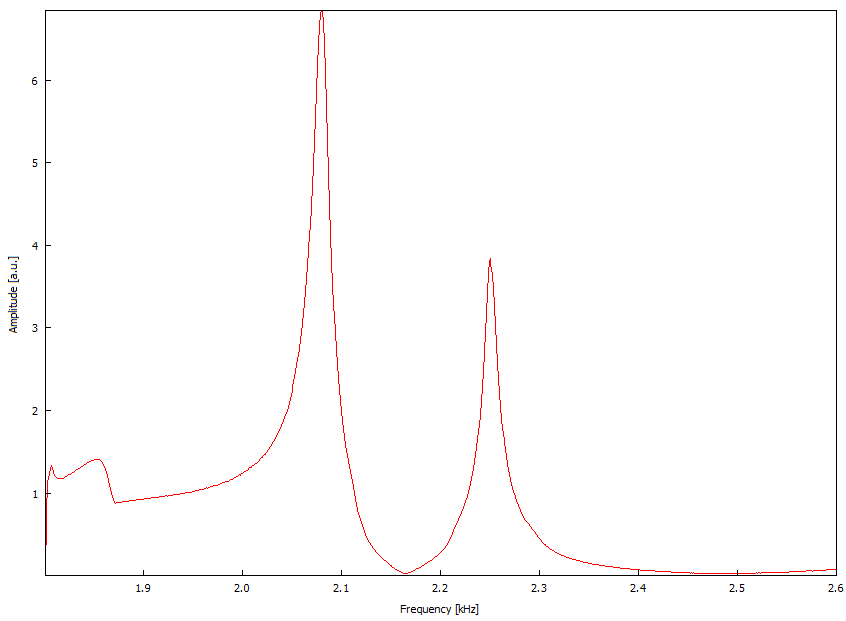
\includegraphics[width=\textwidth]{data/2_4/9mm.png}
        \caption{9\,mm Ring.}
    \end{subfigure}
    \hfill
    \caption{Frequenzspektrum der Resonanzfrequenz 2. Ordnung des Kugelresonators mit eingesetztem Zwischenring verschiedener Größe.}
    \label{fig:ringe}
\end{figure}
Wie zu sehen ist, spaltet sich der Resonanzpeak in zwei Peaks auf. Dabei variiert die Amplitude 
der Peaks je nach Ringdicke, wobei sich der Abstand beider Peaks mit steigender
Ringdicke auch erhöht. Der Abstand der Frequenzen ist in \autoref{fig:freq_diff} gegen die 
Ringdicke aufgetragen. Des weiteren wurde mittels Python 3.8.0 eine Ausgleichgerade der Form
\begin{equation*}
     \Delta f = a \cdot d + b
\end{equation*}
erstellt. Der Fehler der Frequenzmessung wird dabei als $1$\;Hz angenommen, da dies auch die 
Schrittweite der Frequenz bei dieser Messung ist; die Durchmesser der Ringe werden als genau
angenommen, da sie vom Hersteller angegeben sind. Die Parameter ergeben sich mittels des Paketes
\textit{Numeric Python} \cite{numpy} und die Fehlerrechnung wird allgemein automatisiert 
mittels des Paketes \textit{uncertainties} \cite{uncertainties}.
Die Parameter der Geraden ergeben sich zu 
\begin{align*}
    a &= (18 \pm 1) \;\frac{\text{Hz}}{\text{mm}} \\
    b &= ( 6 \pm 6) \;\text{Hz}.
\end{align*} 
\begin{figure}[h]
    \centering 
    \includegraphics[width=0.6\textwidth]{build/ausgleichsgerade.pdf}
    \caption{Auftragung der Messwerte der Frequenzdifferenz gegen die Ringdicke mit Ausgleichgerade.}
    \label{fig:freq_diff}
\end{figure}

Für den 9\;mm Ring werden zudem die beiden Resonanzpeaks gegen den Azimutwinkel $\varphi$ aufgetragen 
und wiederum mit der entsprechenden Kugelflächenfunktion verglichen. Dies ist in \autoref{fig:9mmpolar}
zu sehen.
\begin{figure}
    \centering
    \begin{subfigure}[b]{0.48\textwidth}
        \centering
        \includegraphics[width=\textwidth]{build/resonanz1.pdf}
        \caption{1. Resonanz.}
    \end{subfigure}
    \hfill
    \begin{subfigure}[b]{0.48\textwidth}
        \centering
        \includegraphics[width=\textwidth]{build/resonanz2.pdf}
        \caption{2. Resonanz.}
    \end{subfigure}
    \hfill
    \caption{Resonanzen der beiden Peaks in Abhängigkeit des Azimutwinkels $\varphi$ mit entsprechenden Kugelflächenfunktionen.}
    \label{fig:9mmpolar}
\end{figure}
Hier folgen die Messwerte den Kugelflächenfunktionen sehr gut, wenngleich kleinere Abweichungen dennoch
vorkommen können. Die beiden Resonanzen stellen somit die $m$-Aufspaltung in $m = 0$ und $m = 1$ dar mit 
$l = 1$. 

\subsection{Das Wasserstoffmolekül}
In diesem Teil werden die Frequenzspektren des Wasserstoffmolekülmodells mit verschiedenen Blenden
(5\;mm, 10\;mm, 15\;mm und 20\;mm Durchmesser), sowie einmal ohne Blende aufgenommen. Der Frequenzbereich
verläuft dabei von 2,2\;kHz bis 2,5\;kHz. Die Spektren sind in \autoref{fig:blenden} beziehungsweise \autoref{fig:ohne} dargestellt.
\begin{figure}
    \centering
    \begin{subfigure}[b]{0.48\textwidth}
        \centering
        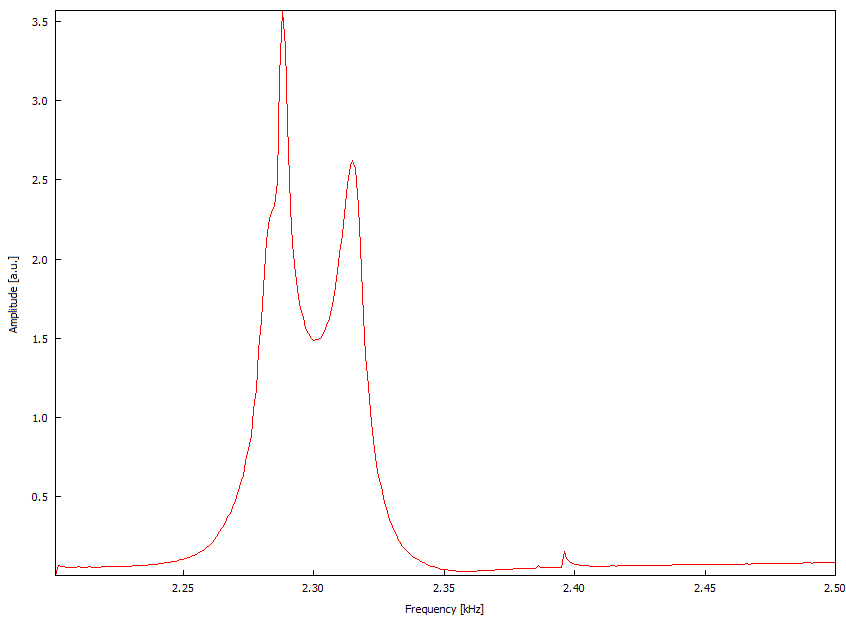
\includegraphics[width=\textwidth]{data/3_1/5mm.png}
        \caption{$d = $ 5\;mm.}
    \end{subfigure}
    \hfill
    \begin{subfigure}[b]{0.48\textwidth}
        \centering
        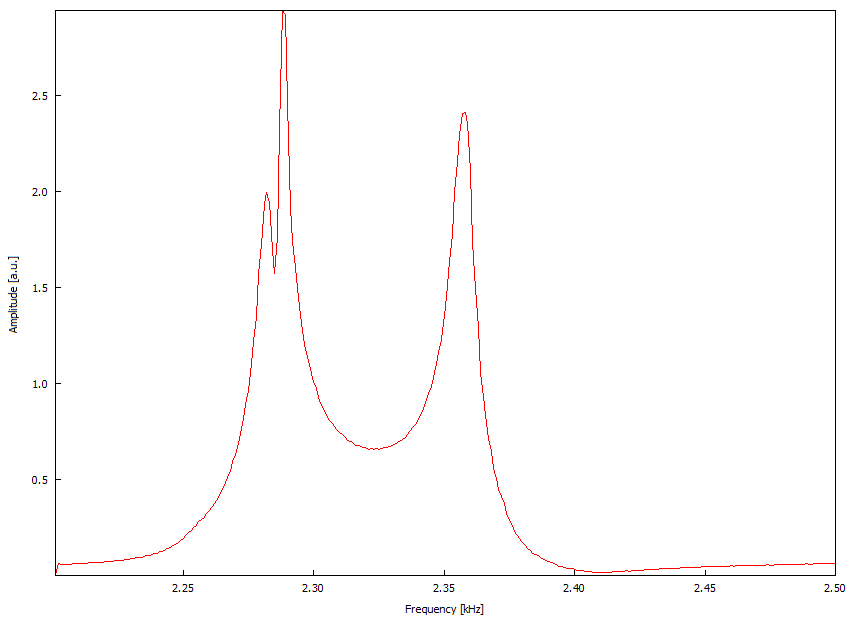
\includegraphics[width=\textwidth]{data/3_1/10mm.png}
        \caption{$d = $ 10\;mm.}
    \end{subfigure}
    \hfill
    \begin{subfigure}[b]{0.48\textwidth}
        \centering
        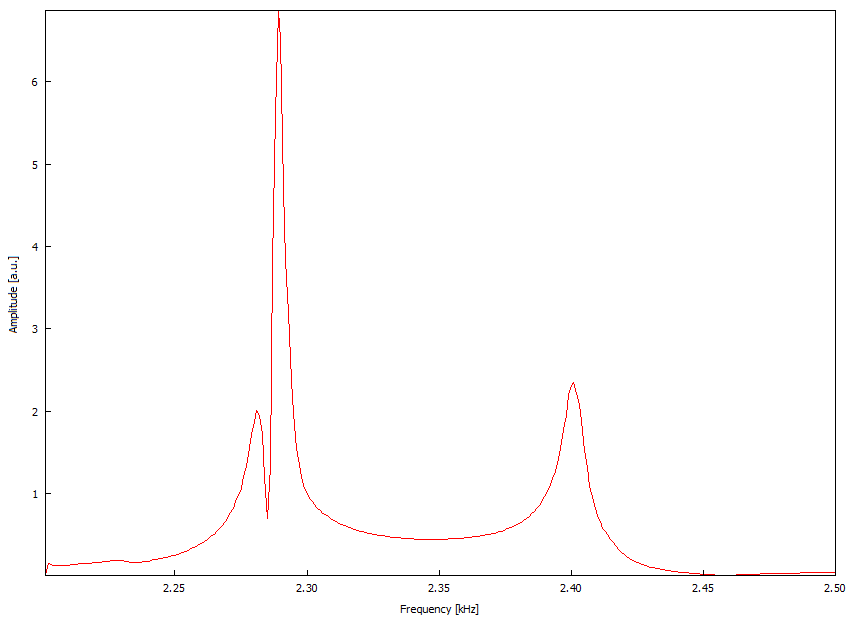
\includegraphics[width=\textwidth]{data/3_1/15mm.png}
        \caption{$d = $ 15\;mm.}
    \end{subfigure}
    \hfill
    \begin{subfigure}[b]{0.48\textwidth}
        \centering
        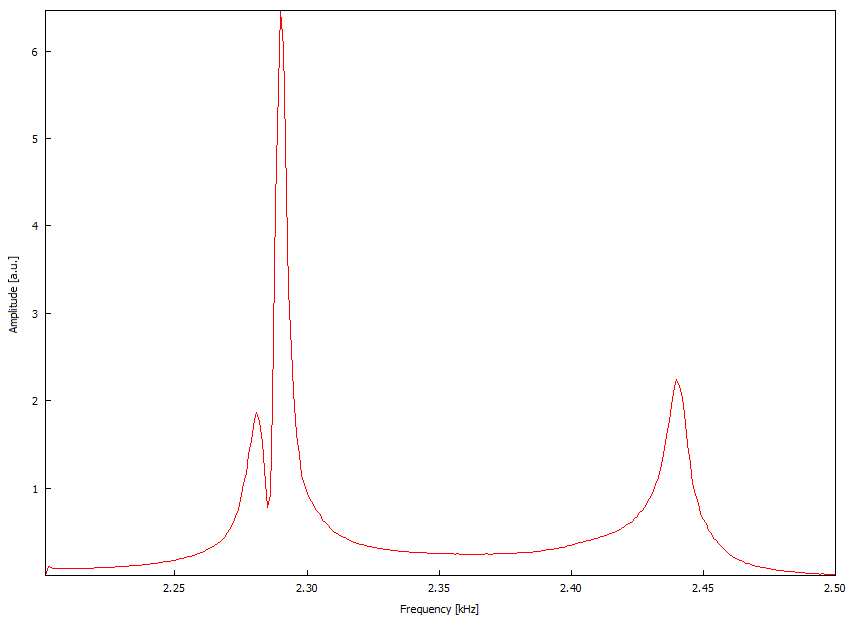
\includegraphics[width=\textwidth]{data/3_1/20mm.png}
        \caption{$d = $ 20\;mm.}
    \end{subfigure}
    \hfill
    \caption{Frequenzspektren des Wasserstoffmolekülmodells (zwei Kugelresonatoren) im Bereich 2,2\;kHz bis 2,5\;kHz mit verschiendenen Blendendurchmessern $d$ zwischen den Kugeln.}
    \label{fig:blenden}
\end{figure}
\begin{figure}
    \centering
    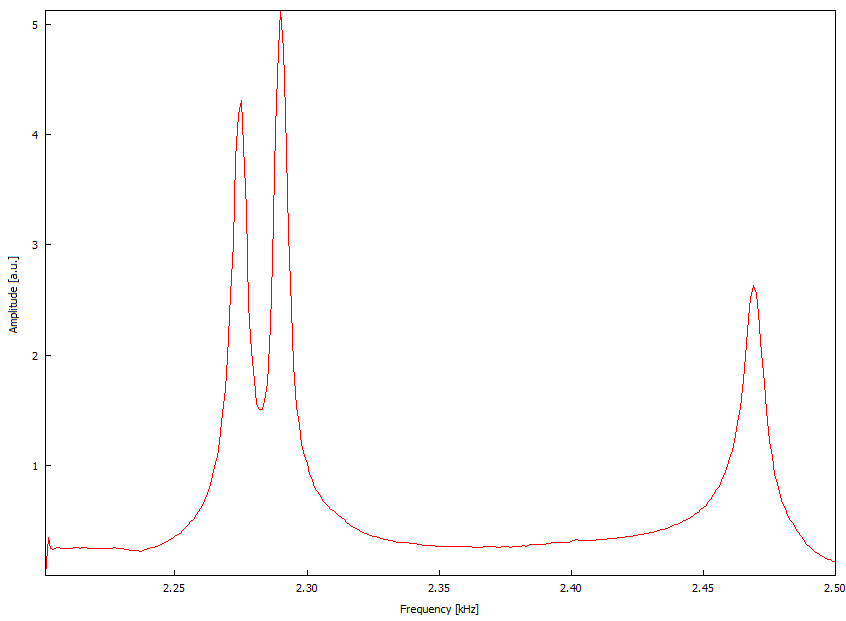
\includegraphics[width=0.5\textwidth]{data/3_1/ohne.png}
    \caption{Frequenzspektren des Wasserstoffmolekülmodells (zwei Kugelresonatoren) im Bereich 2,2\;kHz bis 2,5\;kHz ohne Blende zwischen den Kugeln.}
    \label{fig:ohne}
\end{figure}
Zu sehen sind jeweils drei Peaks, wobei der erste Peak bei der 5\;mm Blende kaum erkennbar ist, 
die jeweils je nach Blendendurchmesser $d$ bei unterschiedlichen Frequenzen liegen. Diese Frequenzen
in Abhängigkeit des Blendendurchmessers sind in \autoref{fig:frequenz_blende} zu sehen.
\begin{figure}
    \centering
    \includegraphics[width=0.5\textwidth]{build/frequenz_blende}
    \caption{Die Resonanzfrequenzen der beiden Kugelresonatoren in Abhängigkeit des Blendendurchmessers $d$.}
    \label{fig:frequenz_blende}
\end{figure} 
Wie schon erwartet sind zwei der Peaks immer sehr nah beieinander, während der dritte, der mit
der höchsten Frequenz, weiter weg ist. Weiterhin ist ein linearer Zusammenhang zwischen
letzteren Peaks und dem Blendendurchmesser $d$ erkennbar. Die Messung ohne Blende fügt sich
diesem Effekt nicht. \\
Die Winkelverteilung der drei Resonanzpeaks ist für die Blende mit 15\;mm Durchmesser aufgenommen worden 
und in \autoref{fig:polar_blende} dargestellt.
\begin{figure}[hp]
    \centering
    \begin{subfigure}[b]{0.48\textwidth}
        \centering
        \includegraphics[width=\textwidth]{blende_polar1.pdf}
        \caption{1. Resonanz.}
    \end{subfigure}
    \hfill
    \begin{subfigure}[b]{0.48\textwidth}
        \centering
        \includegraphics[width=\textwidth]{blende_polar2.pdf}
        \caption{2. Resonanz.}
    \end{subfigure}
    \hfill
    \begin{subfigure}[b]{0.48\textwidth}
        \centering
        \includegraphics[width=\textwidth]{blende_polar3.pdf}
        \caption{3. Resonanz.}
    \end{subfigure}
    \hfill
    \caption{Verteilung der Peaks der drei beobachteten Resonanzen an den zwei Kugelresonatoren mit einem Blendendurchmesser von 15\;mm  in Abhängigkeit des Azimutwinkels $\varphi$.}
    \label{fig:polar_blende}
\end{figure}
Es werden insgesamt 3 Resonanzen detektiert. Auffällig ist das konstante Verhalten der Amplitude
der dritten Resonanz, während die anderen beiden Peaks in ihrer Amplitude schwanken, aber ähnliche
Verläufe zeigen. Dies ist schon Indiz dafür, dass der eine Peak den anderen überlagert. \\
Die Phasendifferenz zwischen unterer und ober Kugel an den Resonanzfrequenzen ist in \autoref{tab:phasediff}
aufgetragen.
\begin{table}[!htp]
    \centering
    \caption{Phasendifferenzen zwischen ober und unterer Kugel an den Resonanzfrequenzen an den zwei Kugelresonatoren.}
    \label{tab:phasediff}
    \begin{tabular}{c c c}
    \toprule
    {Peak Nummer} & {Resonanzfrequenz / kHz} & {Absolute Phasendifferenz / °}\\
    \midrule 
    1  & 2,28 & 180\\ 
    2  & 2,293 & 218   \\
    3  & 2,472 &180  \\
    \bottomrule
    \end{tabular}
    \end{table}
Auffällig ist, dass beim zweiten Peak eine Phasendifferenz deutlich größer als 180$°$ gemessen wurde.
Der Zustand, der hier letztlich vermessen wurde, ist beim dritten Peak der Zustand $ 2 \sigma_{\text{u}}$.
Die anderen beiden Peaks sollten theoretisch die Zustände $2 \sigma_{\text{g}}$ und 
$1 \pi_{\text{u}}$ zeigen. Diese überlagern sich allerdings so, dass keine genauere Bestimmung möglich ist.

\subsection{Der eindimensionaler Festkörper}
Zunächst wird eine Kette aus gleichen Elementarzellen und gleichen Streuzentren simuliert.
Dazu ist zunächst das Frequenzspektrum von 0,1\;kHz bis 12\;Hz von 50\;mm Zylindern und
Irisblenden mit 16\;mm Durchmesser dargestellt. Exemplarisch sind dies die Spektren mit 
2, 4 und 10 Zylindern in \autoref{fig:allesgleich} dargestellt. Die übrigen Spektren sind im 
Anhang als \autoref{fig:anhang_allesgleich} aufgeführt. 
\begin{figure}
    \centering
    \begin{subfigure}[b]{0.3\textwidth}
        \centering
        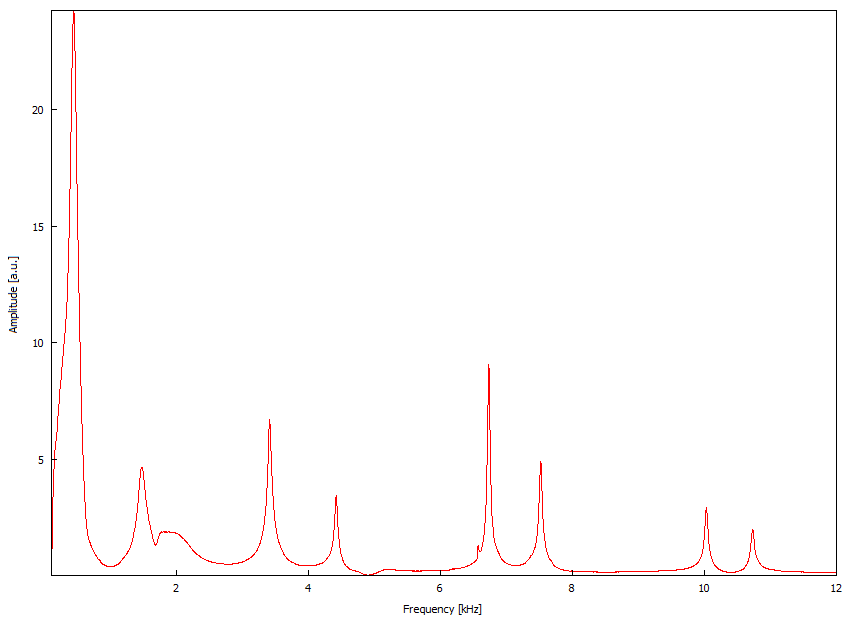
\includegraphics[width=\textwidth]{data/4_1/2.png}
        \caption{2 Zylinder.}
    \end{subfigure}
    \hfill
    \begin{subfigure}[b]{0.3\textwidth}
        \centering
        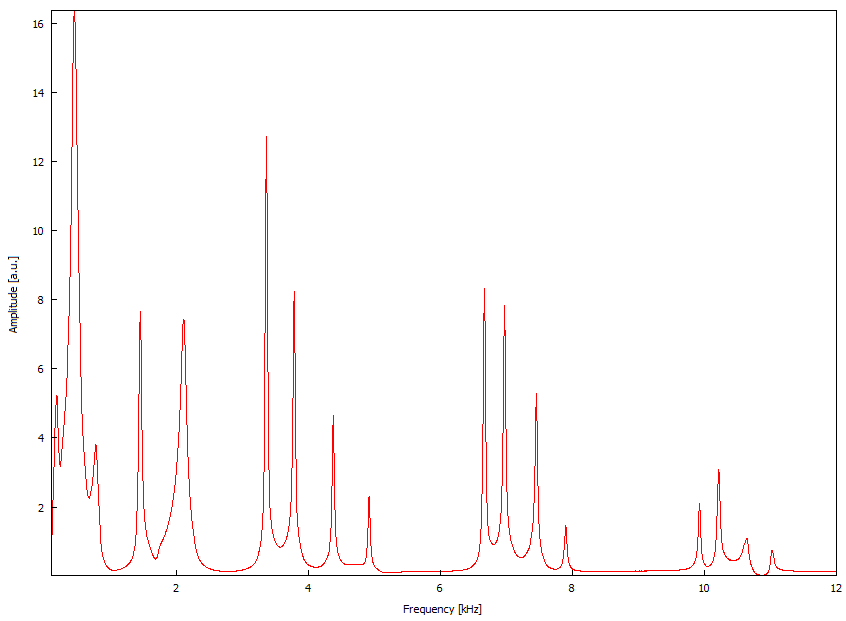
\includegraphics[width=\textwidth]{data/4_1/4.png}
        \caption{4 Zylinder.}
    \end{subfigure}
    \hfill
    \begin{subfigure}[b]{0.3\textwidth}
        \centering
        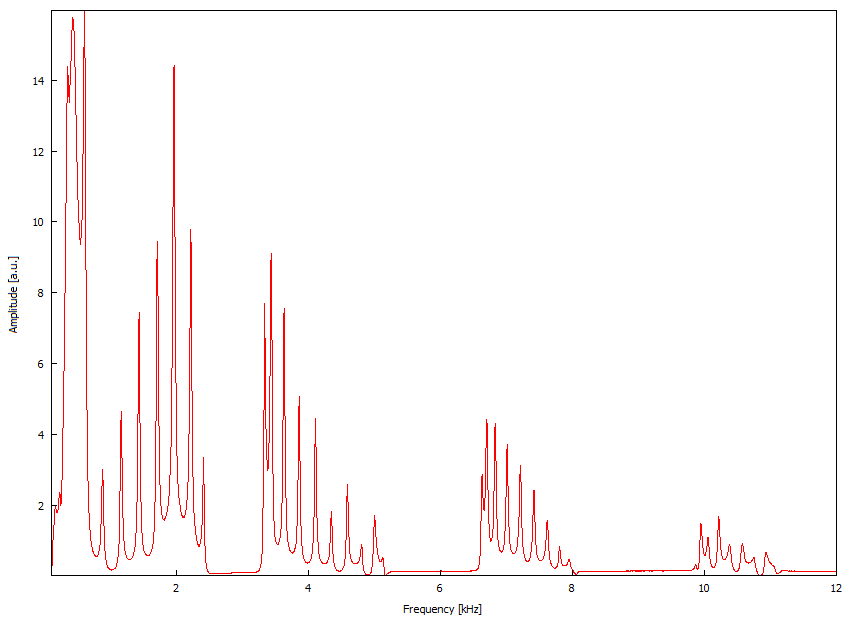
\includegraphics[width=\textwidth]{data/4_1/10.png}
        \caption{10 Zylinder.}
    \end{subfigure}
    \hfill
    \caption{Frequenzspektrum von verschiedener Anzahl von Zylinder mit 50\;mm Länge und jeweils Irsiblenden mit 16\;mm Durchmesser dazwischen im Bereich 0,1\;kHz bis 12\;Hz.}
    \label{fig:allesgleich}
\end{figure}
Scheinbar steigt die Anzahl der Resonanzfrequenzen mit der Anzahl der Zylinder an. Die Resonanzen scheinen sich in
Gruppen anzuordnen, in denen immer so viele Peaks wie Zylinder sind. Der Abstand der Peaks nimmt
dabei generell ab. Ähnliche Spektren sind auch für Irisblenden mit 10\;mm und 13\;mm Durchmesser 
in \autoref{fig:allesgleich10} und \autoref{fig:allesgleich13} zu sehen.
\begin{figure}
    \centering
    \begin{subfigure}[b]{0.3\textwidth}
        \centering
        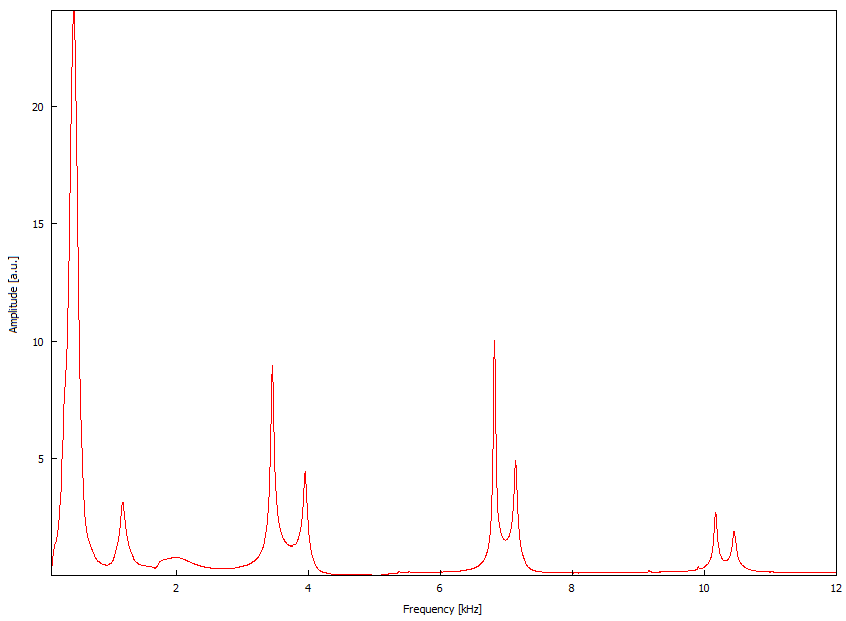
\includegraphics[width=\textwidth]{data/4_2/10mm_2zylinder.png}
        \caption{2 Zylinder.}
    \end{subfigure}
    \hfill
    \begin{subfigure}[b]{0.3\textwidth}
        \centering
        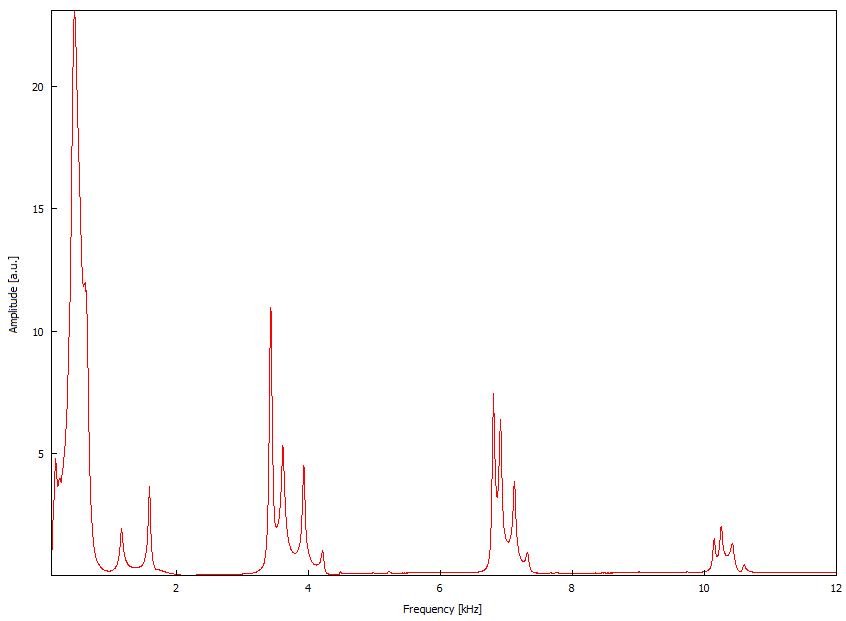
\includegraphics[width=\textwidth]{data/4_2/10mm_4zylidner.png}
        \caption{4 Zylinder.}
    \end{subfigure}
    \hfill
    \begin{subfigure}[b]{0.3\textwidth}
        \centering
        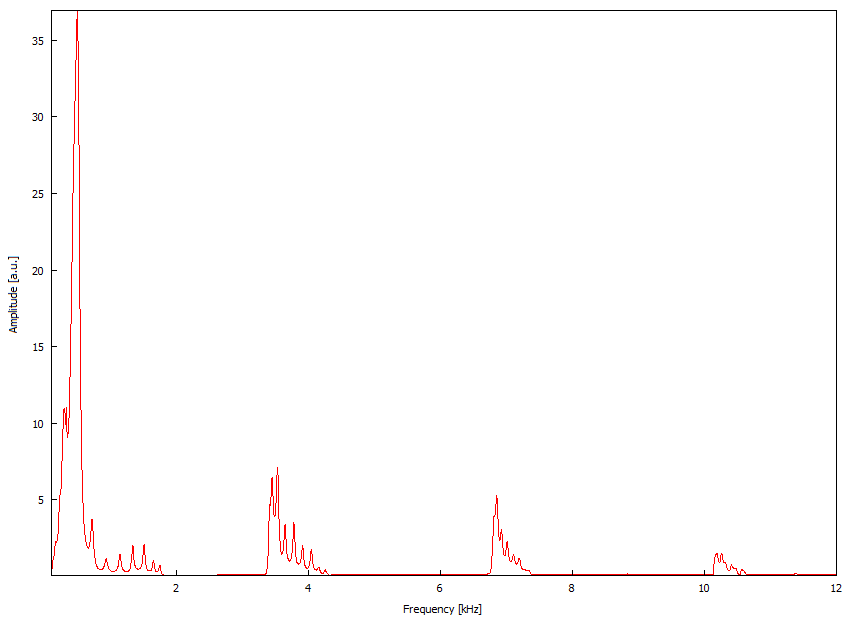
\includegraphics[width=\textwidth]{data/4_2/10mm_10zylinder.png}
        \caption{10 Zylinder.}
    \end{subfigure}
    \hfill
    \caption{Frequenzspektrum bei verschiedener Anzahl von Zylinder mit 50\;mm Länge und jeweils Irsiblenden mit 10\;mm Durchmesser dazwischen im Bereich 0,1\;kHz bis 12\;Hz.}
    \label{fig:allesgleich10}
\end{figure}
\begin{figure}
    \centering
    \begin{subfigure}[b]{0.3\textwidth}
        \centering
        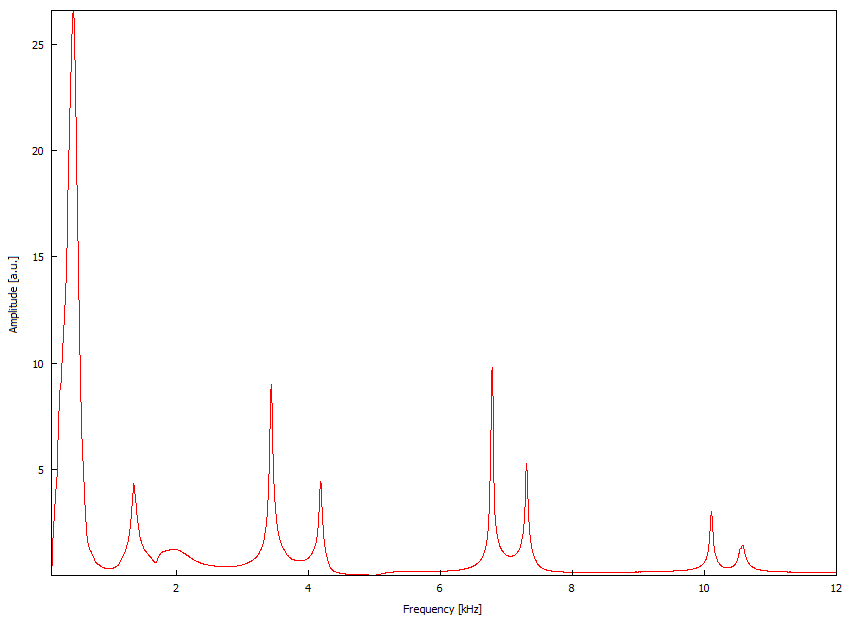
\includegraphics[width=\textwidth]{data/4_2/13mm_2zylinder.png}
        \caption{2 Zylinder.}
    \end{subfigure}
    \hfill
    \begin{subfigure}[b]{0.3\textwidth}
        \centering
        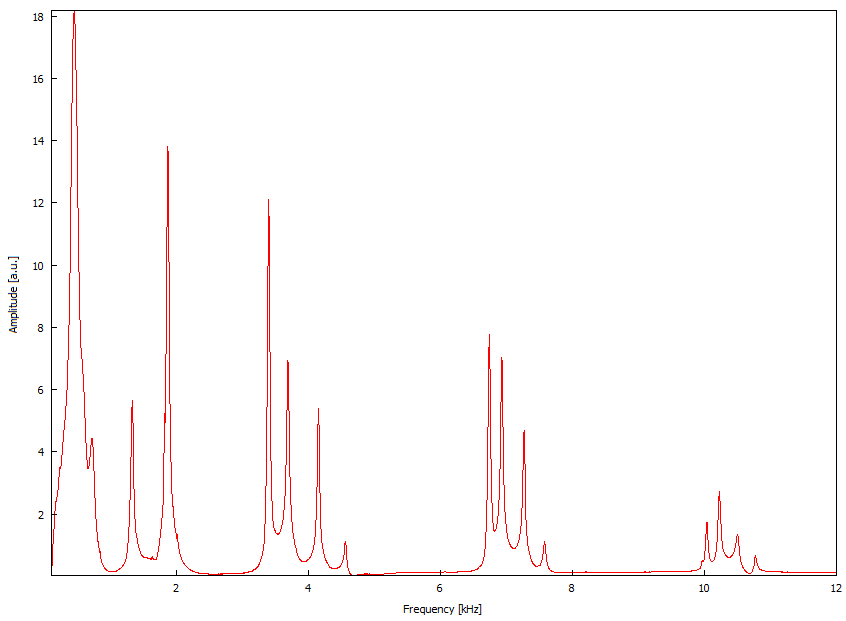
\includegraphics[width=\textwidth]{data/4_2/13mm_4zylinder.png}
        \caption{4 Zylinder.}
    \end{subfigure}
    \hfill
    \begin{subfigure}[b]{0.3\textwidth}
        \centering
        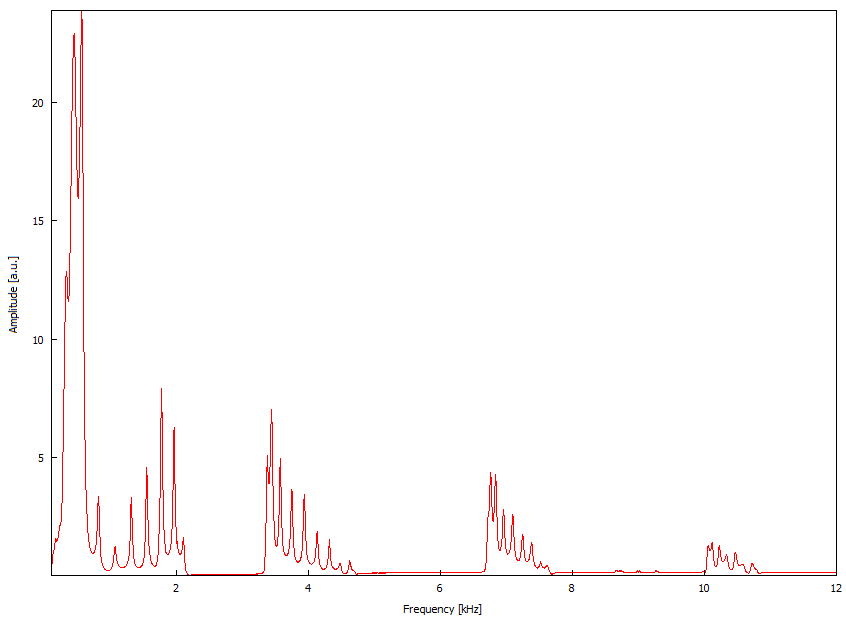
\includegraphics[width=\textwidth]{data/4_2/13mm_10zylinder.png}
        \caption{10 Zylinder.}
    \end{subfigure}
    \hfill
    \caption{Frequenzspektrum von verschiedenen Anzahlen Zylinder mit 50\;mm Länge und jeweils Irsiblenden mit 13\;mm Durchmesser dazwischen im Bereich 0,1\;kHz bis 12\;Hz.}
    \label{fig:allesgleich13}
\end{figure}
Von der Struktur her unterscheiden sich beide Spektren nur geringfügig vom Spektrum mit den 
16\;mm Irisblenden. Die Lücke zwischen den einzelnen Peakgruppen wird allerdings mit kleinerer
Blende größer. Bezogen auf den Festkörper kann diese Lücke als Bandlücke interpretiert werden, 
die bei kleineren Streuzentren größer wird. Die Aufteilung der Peaks innerhalb der Gruppe kann 
durch den Einfluss der Streuung interpretiert werden. Ohne Streuung wäre die Gruppe nur ein großer Peak.\\
In einer 10 zylindrigen Kette aus 50\;mm Zylindern wird ein Zylinder durch einen Zylinder 
einer anderen Größe ersetzt. Die anderen Zylinder haben die Größe 37,5\;mm, 62,5\;mm, sowie 75\;mm.
Die entsprechenden Frequenzspektren sind in \autoref{fig:einzylinderanders} zu sehen.
\begin{figure}
    \centering
    \begin{subfigure}[b]{0.3\textwidth}
        \centering
        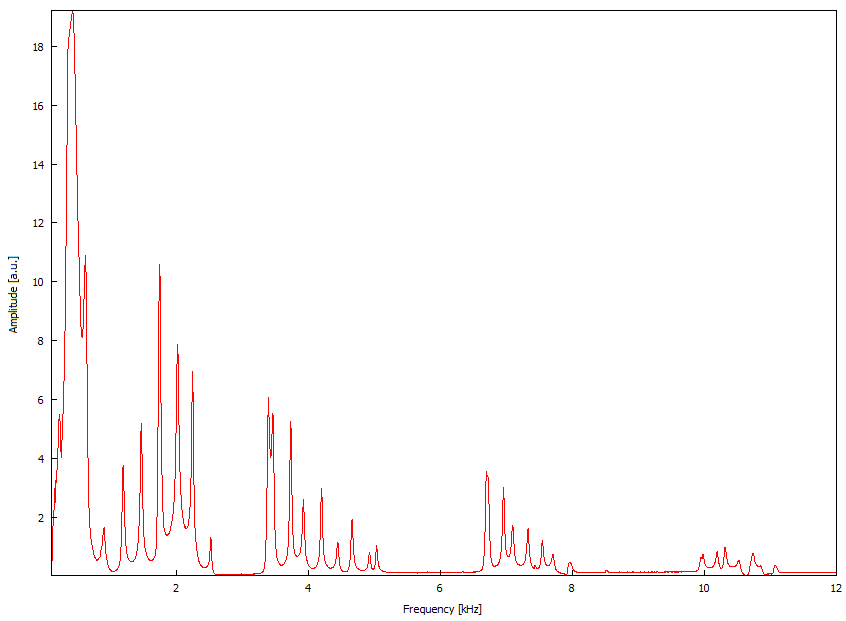
\includegraphics[width=\textwidth]{data/4_3/375.png}
        \caption{$l =$ 37,5\;mm.}
    \end{subfigure}
    \hfill
    \begin{subfigure}[b]{0.3\textwidth}
        \centering
        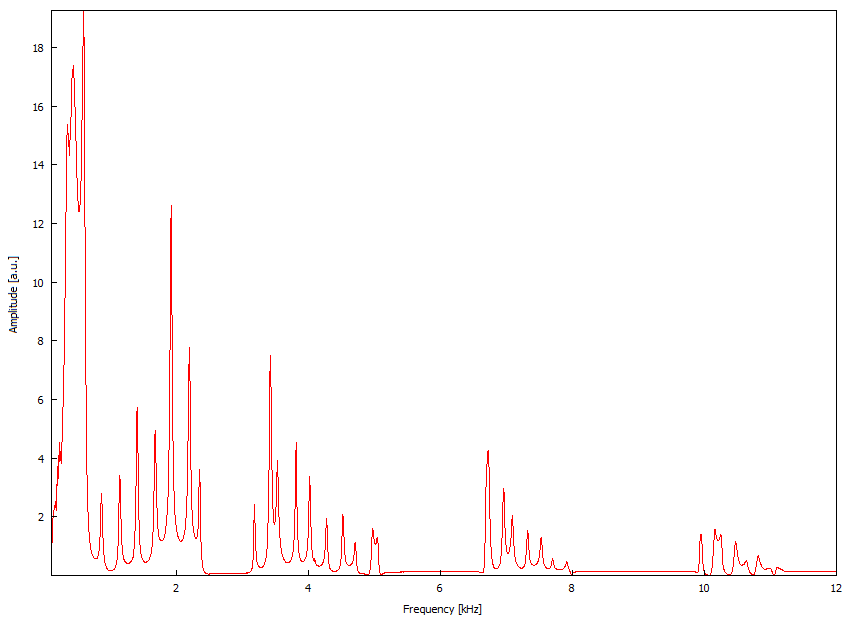
\includegraphics[width=\textwidth]{data/4_3/625mm.png}
        \caption{$l =$ 62,5\;mm.}
    \end{subfigure}
    \hfill
    \begin{subfigure}[b]{0.3\textwidth}
        \centering
        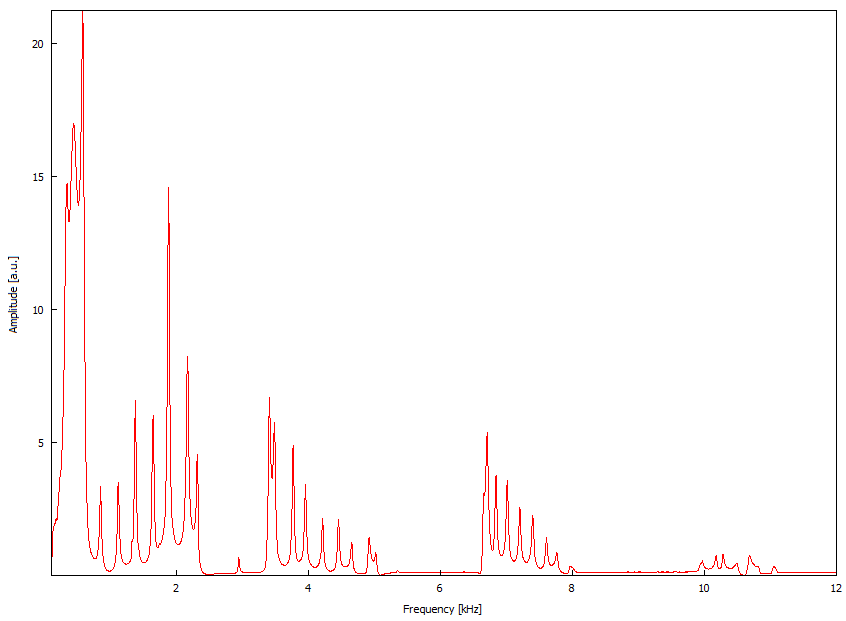
\includegraphics[width=\textwidth]{data/4_3/75mm.png}
        \caption{$l =$ 75\;mm.}
    \end{subfigure}
    \hfill
    \caption{Frequenzspektrum von 9 Zylindern mit $l = $ 50\;mm Länge und einem Zylinder unterschiedlicher Länge und jeweils Irsiblenden mit 16\;mm Durchmesser dazwischen im Bereich 0,1\;kHz bis 12\;Hz.}
    \label{fig:einzylinderanders}
\end{figure}
Für die unterschiedlichen eingesetzten Zylinder verändert sich die Position einer Resonanzfrequenz
an der ersten Bandlücke, beziehungsweise im Falle des 75\;mm Zylinders innerhalb der ersten Bandlücke.\\

Durch Abwechseln der Zylindergrößen (hier: 50\;mm und 75\;mm) lässt sich ein eindimensionaler
Festkörper mit zwei unterschiedlichen Elementarzellen simulieren, wobei die Streuzentren konstant
bleiben (Irsiblenden mit Durchmesser 16\;mm). Das Frequenzspektrum ist in \autoref{fig:abwechselndezylinder}
dargstellt.
\begin{figure}
    \centering
        \centering
        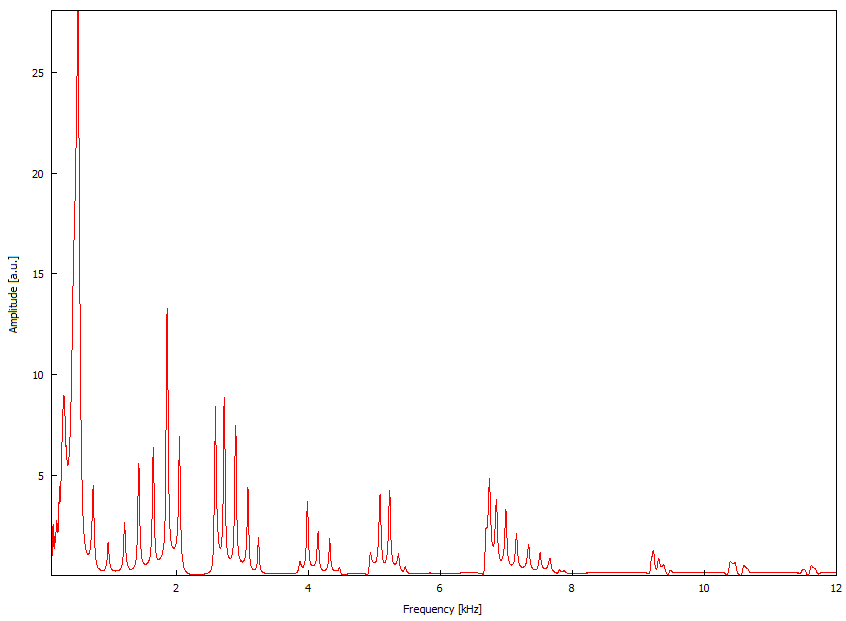
\includegraphics[width=0.55\textwidth]{data/4_4/abwechselnd.png}
    \caption{Frequenzspektrum einer 10 Zylinderkette mit abwechselnd $l = $ 50\;mm und $l = 75$\;mm Länge und jeweils Irsiblenden mit 16\;mm Durchmesser dazwischen im Bereich 0,1\;kHz bis 12\;Hz.}
    \label{fig:abwechselndezylinder}
\end{figure}
Im direkten Vergleich mit dem Spektrum eines einzelnen 50\;mm beziehungsweise 75\;mm Zylinder in 
\autoref{fig:blub1} und \autoref{fig:75mm1} fällt auf, dass es sich tatsächlich um eine Überlagerung 
beider Frequenzspektren handelt. Die zuvor betrachteten Gruppen bestehen im Prinzip aus 
zwei zusammengefügten Gruppen. Es ergeben sich so andere Zustände als in den Zylinderketten zuvor.\\
Durch Beibehalten der Zylinderstruktur (50\:mm) und abwechseln der Irisblenden (16\;mm und 13\;mm)
ergibt sich das Spektrum in \autoref{fig:abwechselndeblenden}.
\begin{figure}
    \centering
        \centering
        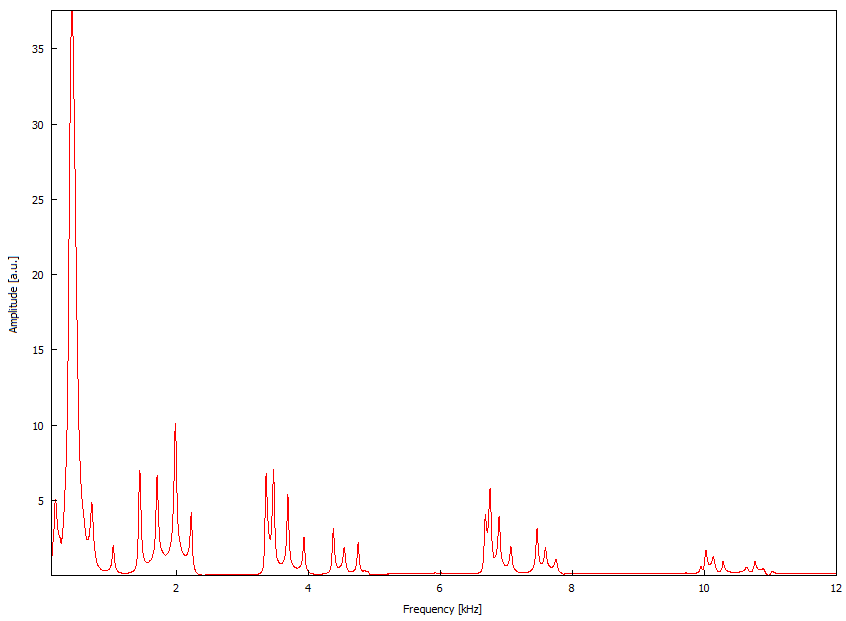
\includegraphics[width=0.55\textwidth]{data/4_5/abwechselndeblende.png}
    \caption{Frequenzspektrum einer 10 Zylinderkette mit Längen $l = $ 50\;mm und jeweils abwechselnd Irsiblenden mit 16\;mm beziehungsweise 13\;mm Durchmesser dazwischen im Bereich 0,1\;kHz bis 12\;Hz.}
    \label{fig:abwechselndeblenden}
\end{figure}
In diesem Fall bilden sich neben den Resonanzgruppen deutlich kleinere Gruppen aus, mit einer Lücke 
dazwischen. Dies kann dahingehend interpretiert werden, dass durch unterschiedliche Sreuzentren
weitere Bänder entstehen.